%!TEX root = SISC_elastic_3d.tex
\subsection{Iterative methods}\label{iterative_section}
In this section, we use the same example as in Sec.~\ref{convergence_study}. For the proposed scheme (\ref{elastic_semi_c}, \ref{fine_scheme}, \ref{continuous_sol}, \ref{continuous_traction}), we need to solve a $3n_1^{2h}n_2^{2h}\times 3n_1^{2h}n_2^{2h}$ linear system at each time step twice for the continuity of traction at the interface $\Gamma$. 

We investigate three iterative methods: the block Jacobi method, the conjugate gradient method, and the preconditioned conjugate gradient method. We note that the coefficient matrix of the linear system arising from the continuity of traction at interface $\Gamma$ is not symmetric positive definite for this test problem. However, our experiment shows that both the conjugate gradient method and the preconditioned conjugate gradient method converge. Except the following test that compares the three iterative methods, we always use the block Jacobi method to guarantee that the whole scheme converges. 

For the problem proposed in Sec.~\ref{convergence_study}, the structure of the coefficient matrix of the linear system arising in (\ref{continuous_traction}) is shown in Figure \ref{Mass_matrix}, which is determined by the interpolation operator ${\mathcal{P}}$ and restriction operator ${\mathcal{R}}$. Here, we use $n_1^{2h} = n_2^{2h}=13, n_3^{2h} = 7$ as an example. We choose the red parts in Figure \ref{Mass_matrix} to be the block Jacobi matrix in block Jacobi iterative method and preconditioning matrix in preconditioned conjugate gradient iterative method. The absolute error tolerance is set to be $1e-7$ for all three iterative methods and $h_1 = h_2 = h_3 = h$.

\begin{table}[htbp]
	\begin{center}
		\begin{tabular}{|c|c c c|}
			\hline
			$2h$   & ~~~~ CG ~~~~& Block Jacobi & Preconditioned CG  \\
			\hline
			$2\pi/24$ &37.78& 24.96& 4.01\\
			\hline
			$2\pi/48$ &38.61 & 25.38 & 2.87\\
			\hline 
			$2\pi/96$ &39.14 &25.43 & 2.25\\
			\hline
		\end{tabular}
	\end{center}
	\caption{Condition number of matrices in conjugate gradient method, block Jacobi method and preconditioned conjugate gradient method}\label{condition_number}
\end{table} 
Table \ref{condition_number} shows the condition number of the original coefficient matrix, the block Jacobi matrix and the coefficient matrix after applying the preconditioner, respectively. We observe that the condition number for preconditioned conjugate gradient method is smallest which is consistent with the results of iteration number for different iterative methods: there are around $44$ iterations for conjugate gradient method, $13$ iterations for block Jacobi method and $9$ iterations for preconditioned conjugate gradient method.

In comparison, we have also performed an LU factorization for the linear system when the mesh size $2h = 2\pi/96$, and the computation takes 40.6 GB memory. In contrast, with the block Jacobi method, the peak memory usage is only 1.2 GB. For large-scale problems, the memory usage becomes infeasible for the LU factorization. 

\begin{figure}[H]
	\centering
	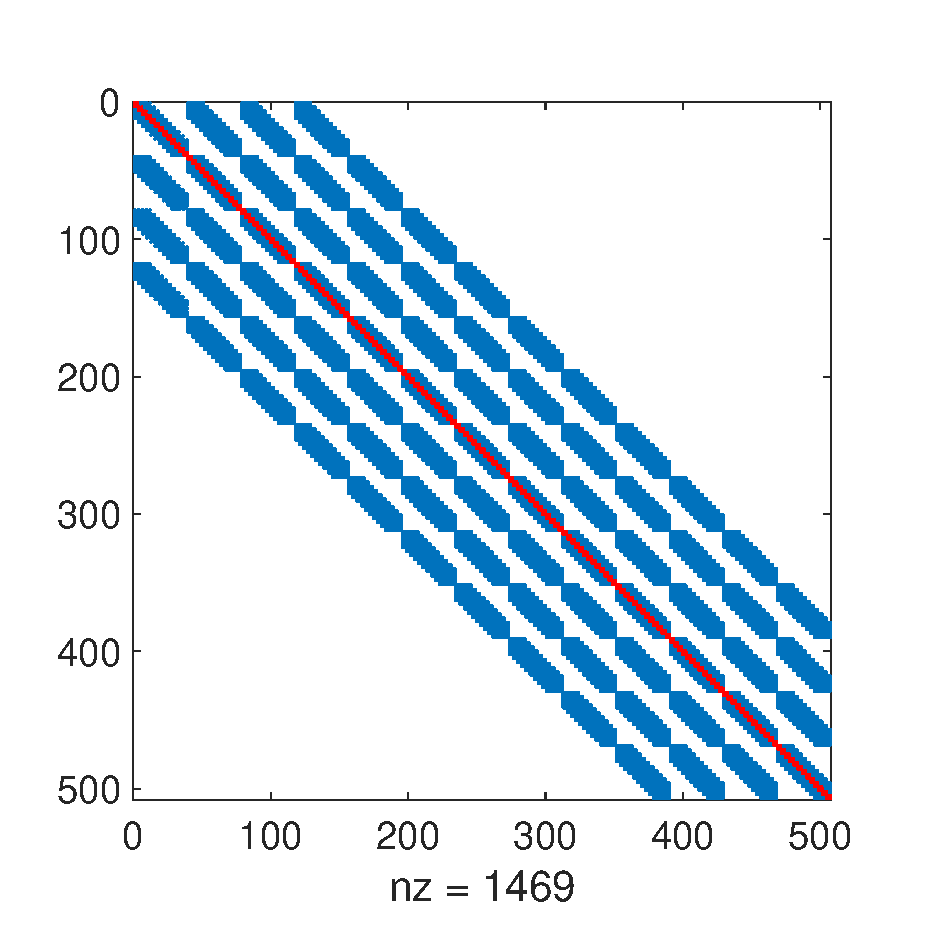
\includegraphics[width=0.45\textwidth,trim={0.6cm 1cm 1cm 1.2cm}, clip]{Mass_matrix.eps}
	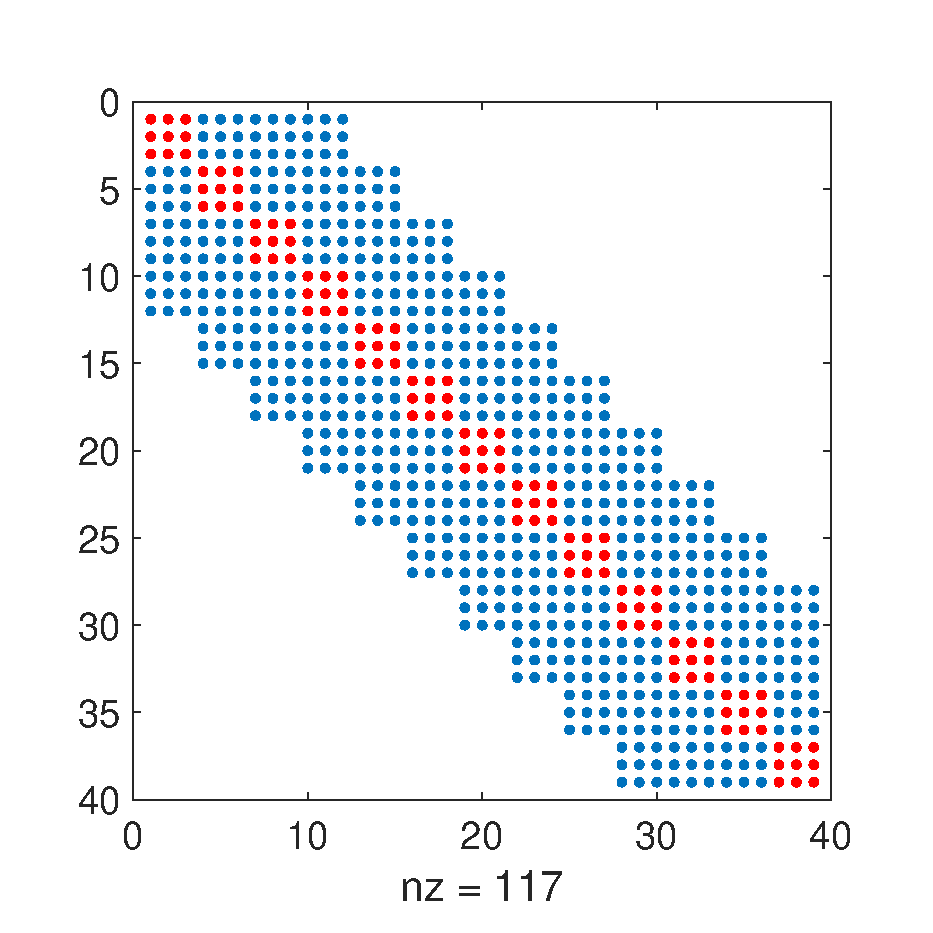
\includegraphics[width=0.45\textwidth,trim={0.6cm 1cm 1cm 1.2cm}, clip]{Mass_diagonal_matrix.eps}
	\caption{The left panel is the structure of the coefficient matrix of the linear system (\ref{continuous_traction}).  The right panel shows a close-up of one diagonal block.}\label{Mass_matrix}
\end{figure}
